\DiaryEntry{Quadratic Reciprocity, Proof}{2022-02-27}{Number Theory}

The proof of the Quadratic Reciprocity Law is based on Gauss's lemma \ref{2023-02-13:th4} and the following lemma.

\begin{theorem}
    If $p$ is an odd prime and $a$ an odd integer with $\gcd(a,p)=1$, then

    \begin{equation*}
        (a/p) = (-1)^{\sum_{k=1}^{(p-1)/2} [ka/p]}
    \end{equation*}

    Be careful, $[ \cdot ]$ denotes the greatest integer function!
\end{theorem}

As an example, consider $(5/11$). The upper limit of the sum is $(p-1)/2 = 5$ and we therefore have to sum

\begin{align*}
\sum_{k=1}^{(p-1)/2} \left[ \frac{ka}{p} \right] &= \left[ \frac{1 \cdot 5}{11} \right] + \left[ \frac{2 \cdot 5}{11} \right] + \left[ \frac{3 \cdot 5}{11} \right] + \left[ \frac{4 \cdot 5}{11} \right] + \left[ \frac{5 \cdot 5}{11} \right] \\
&= 0 + 0 + 1 + 1 + 2 = 4
\end{align*}

and therefore $(5/11) = (-1)^4 = -1$.

\paragraph{Proof.} The underlying idea is to find a closed-form expression for $n$ in Gauss's lemma and use this to calculate $(a/n)$. We start with the set $S = \{a, 2a, 3a, \cdots, \frac{p-1}{2}a \}$ and divide each number by $p$ to obtain

\begin{equation*}
    ka = q_k p + t_k, \quad 1 \leq t_k \leq p-1
\end{equation*}

We can rewrite this as $ka/p = q_k + t_k / p$ and therefore $[ka/p] = q_k$. So we can write (for $1 \leq k \leq (p-1)/2$),

\begin{equation*}
    ka = \left[ \frac{ka}{p} \right] p + t_k
\end{equation*}

where $t_k$ is the remainder. In the proof of Gauss's lemma we split the remainders into two sets: (i) the set $r_1, \ldots, r_m$ as the remainders $t_k$ upon division by $p$ smaller than $p/2$ and (ii) the set $s_1, \ldots, s_n$ as the remainders $t_k$ upon division by $p$ larger than $p/2$. If a reminder $t_k < p/2$, then it is one of the integers $r_k$, otherwise it is one of the integers $s_k$.

Summing up the $(p-1)/2$ equations, we obtain

\begin{equation}\label{2023-02-27:eq1}
    \sum_{k=1}^{(p-1)/2} ka = \sum_{k=1}^{(p-1)/2} \left[ \frac{ka}{p} \right] p + \sum_{k=1}^m r_k + \sum_{k=1}^n s_k
\end{equation}

In proving Gauss's lemma, we showed that the $(p-1)/2$ numbers $r_1, \ldots, r_m, s_1, \ldots, p - s_n$ are just an rearrangement of the integers $1, 2, \ldots, (p-1)/2$. Therefore,

\begin{equation*}
    \sum_{k=1}^{(p-1)/2} k  = \sum_{k=1}^m r_k + \sum_{k=1}^n (p - s_k) = pn + \sum_{k=1}^m r_k - \sum_{k=1}^n s_k
\end{equation*}

Subtracting this from \eqref{2023-02-27:eq1}, we obtain

\begin{equation*}
    (a-1) \sum_{k=1}^{(p-1)/2} k = p \left( \sum_{k=1}^{(p-1)/2} \left[ \frac{ka}{p} \right] - n \right) + 2\sum_{k=1}^m s_k 
\end{equation*}

We can now use the fact that $p \equiv a \mod 2$ to translate the last equation into a congruence relation. The relation $p \equiv a \mod 2$ means that either $a$ and $p$ are odd or even. Since $p$ is a prime, it is odd, therefore $a$ is also odd. This implies $a-1$ is even and let's now write down the remainders after division by $2$,

\bee
0 \cdot \sum_{k=1}^{(p-1)/2} k \equiv 1 \cdot \left( \sum_{k=1}^{(p-1)/2} \left[ \frac{ka}{p} \right] - n \right) + 0 \mod 2
\eee

This is equivalent to

\bee
n \equiv \sum_{k=1}^{(p-1)/2} \left[ \frac{ka}{p} \right] \mod 2
\eee

Having a closed-form expression for $n$, we can now use Gauss's lemma to express $(a/n)$,

\bee
(a/p) = (-1)^n = (-1)^{\sum_{k=1}^{(p-1)/2} [ka/p]} \qed
\eee

With this in place, we can now prove the Quadratic Reciprocity Law. As a reminder, it states that for $p, q$ to be two distinct odd primes, we have

\bee
(p/q)(q/p) = (-1)^{\frac{p-1}{2} \frac{q-1}{2} }
\eee

\paragraph{Proof.} The underlying idea of the proof is to count the number of lattice points in a rectangle of length $p/2$ and $q/2$ as shown in the following Figure. Let $R$ denote the region within this rectangle, not including any of the bounding lines.

\begin{figure}[H]
    \centering
    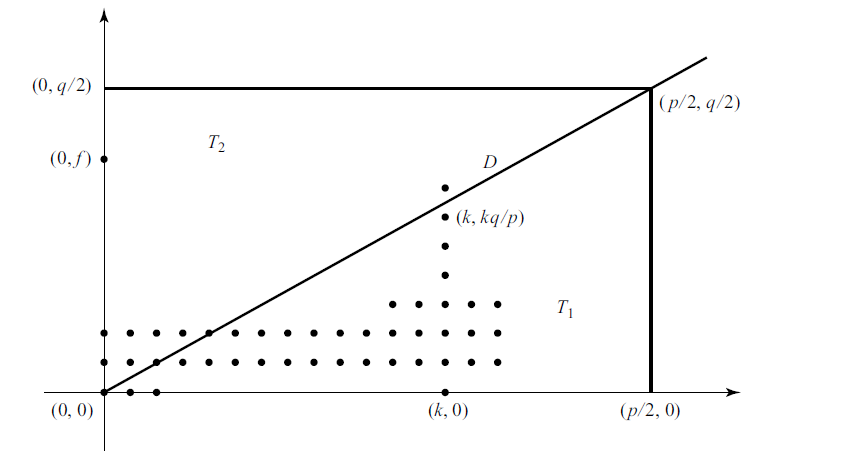
\includegraphics[scale=0.75]{images/2023_02_27_quadr_reci_01.png}
\end{figure}

Because $p$ and $q$ are both odd, the lattice points in $R$ consist of all points $(n,m)$ where $1 \leq n \leq (p-1)/2$ and $1 \leq m \leq (q-1)/2$ and the number of such points is clearly

\be\label{2023-02-27:eq1}
\frac{p-1}{2} \cdot \frac{q-1}{2}
\ee

Let's use a different counting argument. The diagonal $D$ from $(0,0)$ to $(p/2,q/2)$ has the equation $y = (q/p)x$ or $py = qx$. Because $p, q$ are two distinct primes, we have $\gcd(p,q) = 1$ and therefore none of the lattice points inside $R$ will lie on $D$: For $p$ must divide the $x$- coordinate of any lattice point on the line $py = qx$, and $q$ must divide its $y$-coordinate; there are no such points in $R$.

Let $T_1$ denote the portion of $R$ that is below the diagonal $D$, and let $T_2$ denote the portion above. By what we have just seen, it suffices to count the lattice points inside each of these triangles.

Let's fix the $x$-coordinate as $x=k$ and count how many lattice points there are on the line $(k,0)$ and $(k, kq/p)$. There are 

\bee
\left[ \frac{kq}{p} \right]
\eee

such points. Summing along all allowed values for $x$, we obtain for the number of lattice points in $T-1$,

\be\label{2023-02-27:eq2}
\sum_{k=1}^{(p-1)/2} \left[ \frac{kq}{p} \right]
\ee

We can use an analoguous argument to count the number of lattice points in $T-2$ which turns out to be 

\be\label{2023-02-27:eq3}
\sum_{j=1}^{(q-1)/2} \left[ \frac{jp}{q} \right]
\ee

Before we argued that no lattice points will lie on the Diagonal $D$ itself, so the total number of lattice points in $R$ is the sum of the two previvous expressions, \eqref{2023-02-27:eq2} and \eqref{2023-02-27:eq3}. But we have also calculated the number of lattice points in \eqref{2023-02-27:eq1} and we therefore have

\bee
\frac{p-1}{2} \cdot \frac{q-1}{2} = \sum_{k=1}^{(p-1)/2} \left[ \frac{kq}{p} \right] + \sum_{j=1}^{(q-1)/2} \left[ \frac{jp}{q} \right]
\eee

We can now use Gauss's lemma

\begin{align*}
(p/q)(q/p) &= (-1)^{ \sum_{j=1}^{(q-1)/2} \left[ \frac{jp}{q} \right] } \cdot (-1)^{ \sum_{k=1}^{(p-1)/2} \left[ \frac{kq}{p} \right] } \\
&= (-1)^{ \sum_{j=1}^{(q-1)/2} \left[ \frac{jp}{q} \right] + \sum_{k=1}^{(p-1)/2} \left[ \frac{kq}{p} \right] } \\
&= (-1)^{ \frac{p-1}{2} \cdot \frac{q-1}{2} } \qed
\end{align*}

So far so good. According to \cite{Burton2011} it is a very deep result ("For those who consider the theory of numbers “the Queen of Mathematics,” the Quadratic Reciprocity Law is one of the jewels in her crown.") but somehow the deepness / importance is a bit lost on me .-(

Anyway, we have the following corollary: If $p, q$ are two distinct odd primes, then

\bee
(p/q)(q/p) = \begin{cases} 1 & \text{ if } p \equiv 1 \mod 4 \text{ or } q \equiv 1 \mod 4 \\
-1 & \text{ if } p \equiv q \equiv 3 \mod 4 \end{cases}
\eee

We prove this by noting that $(p-1)/2 \cdot (q-1)/2$ is even iff at least one of the integers $p, q$ is of the form $4k+1$. Assume that $p=4k+1$ and $q$ is any odd number, $q=2m+1$. Then

\bee
\frac{p-1}{2} \frac{q-1}{2} = \frac{4k}{2} \frac{2m}{2} = 2k \cdot m
\eee

and this even, independent of $m$. On the other hand, if $p=4k+3$ and $q=4m+3$, then 

\bee
\frac{p-1}{2} \frac{q-1}{2} = \frac{4k+2}{2} \frac{4m + 2}{2} = (2k+1)(2m+1)
\eee

which is odd, independent of $k, m$. \qed

If we take the Quadratic Reciprocity Law and multiply both sides with $(q/p)$, we obtain

\bee
(p/q)(q/p)^2 = (-1)^{\frac{p-1}{2} \frac{q-1}{2} } (q/p)
\eee

We know that $(p/q)^2 = 1$, so we further have

\bee
(p/q) = (-1)^{\frac{p-1}{2} \frac{q-1}{2} } (q/p)
\eee

and from the arguments from above, we know when $\frac{p-1}{2} \frac{q-1}{2}$ is even/odd. Therefore, we have the following theorem.

\begin{theorem}\label{2023-02-27:th1}
For two distinct odd primes $p, q$, we have

\bee
(p/q) = \begin{cases} (q/p) & \text{ if } p \equiv 1 \mod 4 \text{ or } q \equiv 1 \mod 4 \\
- (q/p) & \text{ if } p \equiv q \equiv 3 \mod 4 \end{cases}
\eee
\end{theorem}

We can use this last result to calculate $(a/p)$  with $p$ an odd prime and $a \neq \pm 1$ as not divisible by $p$. Suppose that $a$ can be factored as

\bee
a = \pm 2^{k_0} p_1^{k_1} p_2^{k_2} \cdots p_r^{k_r} 
\eee

The Legendre symbol is multiplicative, so we have

\bee
(a/p) = (\pm 1 /p)(2/p)^{k_0} (p_1/p)^{k_1} (p_2/p)^{k_2} \cdots (p_r/p)^{k_r} 
\eee

We have covered calculation of $(\pm 1 /p)$ and $(2/p)$ before, calculation of $(p_i/p)$ (with $p_i$ and $p$ two distinct odd primes) can be simplified by means of the Quadratic Reciprocity Law as will be shown in the following example.

\paragraph{Example.} Let's calculate $(24/29)$. With $24 = 2^3 \cdot 3$ we have

\bee
(24/29) = (2/29)^3 (3/29)
\eee

By \ref{2023-02-13:th5}, $(2/29) = -1$ because $29 \equiv 5 \mod 8$. In order to calculate $(3/29)$, we invert according to \ref{2023-02-27:th1}. As $q=29 \equiv 1 \mod 4$, we have $(3/29) = (29/3)$. We can simplify this with \ref{2023-02-13:th3}, $(a/p) = (b/p)$ if $a \equiv b \mod p$. So we have $(29/3) = (2/3)$ and with \ref{2023-02-13:th5} again, this becomes $(2/3) = -1$. Combining everything so far, we have

\bee
(24/29) = (-1)^3 (-1) = 1
\eee

Indeed, we have

\begin{verbatim}
from sympy.ntheory import legendre_symbol
from sympy.ntheory import sqrt_mod


print(legendre_symbol(24, 29))
1
print(sqrt_mod(24, 29, all_roots=(True)))
[13, 16]
print(13**2 % 29)
24
print(16**2 % 29)
24
\end{verbatim}
\qed


%%% Local Variables:
%%% mode: latex
%%% TeX-master: "journal"
%%% End:
